\documentclass[]{article}
\usepackage{lmodern}
\usepackage{amssymb,amsmath}
\usepackage{ifxetex,ifluatex}
\usepackage{fixltx2e} % provides \textsubscript
\ifnum 0\ifxetex 1\fi\ifluatex 1\fi=0 % if pdftex
  \usepackage[T1]{fontenc}
  \usepackage[utf8]{inputenc}
\else % if luatex or xelatex
  \ifxetex
    \usepackage{mathspec}
  \else
    \usepackage{fontspec}
  \fi
  \defaultfontfeatures{Ligatures=TeX,Scale=MatchLowercase}
\fi
% use upquote if available, for straight quotes in verbatim environments
\IfFileExists{upquote.sty}{\usepackage{upquote}}{}
% use microtype if available
\IfFileExists{microtype.sty}{%
\usepackage{microtype}
\UseMicrotypeSet[protrusion]{basicmath} % disable protrusion for tt fonts
}{}
\usepackage[margin=1in]{geometry}
\usepackage{hyperref}
\hypersetup{unicode=true,
            pdfborder={0 0 0},
            breaklinks=true}
\urlstyle{same}  % don't use monospace font for urls
\usepackage{color}
\usepackage{fancyvrb}
\newcommand{\VerbBar}{|}
\newcommand{\VERB}{\Verb[commandchars=\\\{\}]}
\DefineVerbatimEnvironment{Highlighting}{Verbatim}{commandchars=\\\{\}}
% Add ',fontsize=\small' for more characters per line
\usepackage{framed}
\definecolor{shadecolor}{RGB}{248,248,248}
\newenvironment{Shaded}{\begin{snugshade}}{\end{snugshade}}
\newcommand{\AlertTok}[1]{\textcolor[rgb]{0.94,0.16,0.16}{#1}}
\newcommand{\AnnotationTok}[1]{\textcolor[rgb]{0.56,0.35,0.01}{\textbf{\textit{#1}}}}
\newcommand{\AttributeTok}[1]{\textcolor[rgb]{0.77,0.63,0.00}{#1}}
\newcommand{\BaseNTok}[1]{\textcolor[rgb]{0.00,0.00,0.81}{#1}}
\newcommand{\BuiltInTok}[1]{#1}
\newcommand{\CharTok}[1]{\textcolor[rgb]{0.31,0.60,0.02}{#1}}
\newcommand{\CommentTok}[1]{\textcolor[rgb]{0.56,0.35,0.01}{\textit{#1}}}
\newcommand{\CommentVarTok}[1]{\textcolor[rgb]{0.56,0.35,0.01}{\textbf{\textit{#1}}}}
\newcommand{\ConstantTok}[1]{\textcolor[rgb]{0.00,0.00,0.00}{#1}}
\newcommand{\ControlFlowTok}[1]{\textcolor[rgb]{0.13,0.29,0.53}{\textbf{#1}}}
\newcommand{\DataTypeTok}[1]{\textcolor[rgb]{0.13,0.29,0.53}{#1}}
\newcommand{\DecValTok}[1]{\textcolor[rgb]{0.00,0.00,0.81}{#1}}
\newcommand{\DocumentationTok}[1]{\textcolor[rgb]{0.56,0.35,0.01}{\textbf{\textit{#1}}}}
\newcommand{\ErrorTok}[1]{\textcolor[rgb]{0.64,0.00,0.00}{\textbf{#1}}}
\newcommand{\ExtensionTok}[1]{#1}
\newcommand{\FloatTok}[1]{\textcolor[rgb]{0.00,0.00,0.81}{#1}}
\newcommand{\FunctionTok}[1]{\textcolor[rgb]{0.00,0.00,0.00}{#1}}
\newcommand{\ImportTok}[1]{#1}
\newcommand{\InformationTok}[1]{\textcolor[rgb]{0.56,0.35,0.01}{\textbf{\textit{#1}}}}
\newcommand{\KeywordTok}[1]{\textcolor[rgb]{0.13,0.29,0.53}{\textbf{#1}}}
\newcommand{\NormalTok}[1]{#1}
\newcommand{\OperatorTok}[1]{\textcolor[rgb]{0.81,0.36,0.00}{\textbf{#1}}}
\newcommand{\OtherTok}[1]{\textcolor[rgb]{0.56,0.35,0.01}{#1}}
\newcommand{\PreprocessorTok}[1]{\textcolor[rgb]{0.56,0.35,0.01}{\textit{#1}}}
\newcommand{\RegionMarkerTok}[1]{#1}
\newcommand{\SpecialCharTok}[1]{\textcolor[rgb]{0.00,0.00,0.00}{#1}}
\newcommand{\SpecialStringTok}[1]{\textcolor[rgb]{0.31,0.60,0.02}{#1}}
\newcommand{\StringTok}[1]{\textcolor[rgb]{0.31,0.60,0.02}{#1}}
\newcommand{\VariableTok}[1]{\textcolor[rgb]{0.00,0.00,0.00}{#1}}
\newcommand{\VerbatimStringTok}[1]{\textcolor[rgb]{0.31,0.60,0.02}{#1}}
\newcommand{\WarningTok}[1]{\textcolor[rgb]{0.56,0.35,0.01}{\textbf{\textit{#1}}}}
\usepackage{longtable,booktabs}
\usepackage{graphicx,grffile}
\makeatletter
\def\maxwidth{\ifdim\Gin@nat@width>\linewidth\linewidth\else\Gin@nat@width\fi}
\def\maxheight{\ifdim\Gin@nat@height>\textheight\textheight\else\Gin@nat@height\fi}
\makeatother
% Scale images if necessary, so that they will not overflow the page
% margins by default, and it is still possible to overwrite the defaults
% using explicit options in \includegraphics[width, height, ...]{}
\setkeys{Gin}{width=\maxwidth,height=\maxheight,keepaspectratio}
\IfFileExists{parskip.sty}{%
\usepackage{parskip}
}{% else
\setlength{\parindent}{0pt}
\setlength{\parskip}{6pt plus 2pt minus 1pt}
}
\setlength{\emergencystretch}{3em}  % prevent overfull lines
\providecommand{\tightlist}{%
  \setlength{\itemsep}{0pt}\setlength{\parskip}{0pt}}
\setcounter{secnumdepth}{0}
% Redefines (sub)paragraphs to behave more like sections
\ifx\paragraph\undefined\else
\let\oldparagraph\paragraph
\renewcommand{\paragraph}[1]{\oldparagraph{#1}\mbox{}}
\fi
\ifx\subparagraph\undefined\else
\let\oldsubparagraph\subparagraph
\renewcommand{\subparagraph}[1]{\oldsubparagraph{#1}\mbox{}}
\fi

%%% Use protect on footnotes to avoid problems with footnotes in titles
\let\rmarkdownfootnote\footnote%
\def\footnote{\protect\rmarkdownfootnote}

%%% Change title format to be more compact
\usepackage{titling}

% Create subtitle command for use in maketitle
\newcommand{\subtitle}[1]{
  \posttitle{
    \begin{center}\large#1\end{center}
    }
}

\setlength{\droptitle}{-2em}
  \title{}
  \pretitle{\vspace{\droptitle}}
  \posttitle{}
  \author{}
  \preauthor{}\postauthor{}
  \date{}
  \predate{}\postdate{}


\begin{document}

\hypertarget{introduction}{%
\section{Introduction}\label{introduction}}

The \texttt{SummarizedExperiment} class is used to store rectangular
matrices of experimental results, which are commonly produced by
sequencing and microarray experiments. Each object stores observations
of one or more samples, along with additional meta-data describing both
the observations (features) and samples (phenotypes).

A key aspect of the \texttt{SummarizedExperiment} class is the
coordination of the meta-data and assays when subsetting. For example,
if you want to exclude a given sample you can do for both the meta-data
and assay in one operation, which ensures the meta-data and observed
data will remain in sync. Improperly accounting for meta and
observational data has resulted in a number of incorrect results and
retractions so this is a very desirable property.

\texttt{SummarizedExperiment} is in many ways similar to the historical
\texttt{ExpressionSet}, the main distinction being that
\texttt{SummarizedExperiment} is more flexible in it's row information,
allowing both \texttt{GRanges} based as well as those described by
arbitrary \texttt{DataFrame}s. This makes it ideally suited to a variety
of experiments, particularly sequencing based experiments such as
RNA-Seq and ChIp-Seq.

\begin{Shaded}
\begin{Highlighting}[]
\KeywordTok{library}\NormalTok{(BiocInstaller)}
\KeywordTok{biocLite}\NormalTok{(}\StringTok{'airway'}\NormalTok{)}
\KeywordTok{biocLite}\NormalTok{(}\StringTok{'SummarizedExperiment'}\NormalTok{)}
\end{Highlighting}
\end{Shaded}

\hypertarget{anatomy-of-a-summarizedexperiment}{%
\section{\texorpdfstring{Anatomy of a
\texttt{SummarizedExperiment}}{Anatomy of a SummarizedExperiment}}\label{anatomy-of-a-summarizedexperiment}}

The \emph{SummarizedExperiment} package contains two classes:
\texttt{SummarizedExperiment} and \texttt{RangedSummarizedExperiment}.

\texttt{SummarizedExperiment} is a matrix-like container where rows
represent features of interest (e.g.~genes, transcripts, exons, etc.)
and columns represent samples. The objects contain one or more assays,
each represented by a matrix-like object of numeric or other mode. The
rows of a \texttt{SummarizedExperiment} object represent features of
interest. Information about these features is stored in a
\texttt{DataFrame} object, accessible using the function
\texttt{rowData()}. Each row of the \texttt{DataFrame} provides
information on the feature in the corresponding row of the
\texttt{SummarizedExperiment} object. Columns of the DataFrame represent
different attributes of the features of interest, e.g., gene or
transcript IDs, etc.

\texttt{RangedSummarizedExperiment} is the ``child''" of the
\texttt{SummarizedExperiment} class which means that all the methods on
\texttt{SummarizedExperiment} also work on a
\texttt{RangedSummarizedExperiment}.

The fundamental difference between the two classes is that the rows of a
\texttt{RangedSummarizedExperiment} object represent genomic ranges of
interest instead of a \texttt{DataFrame} of features. The
\texttt{RangedSummarizedExperiment} ranges are described by a
\texttt{GRanges} or a \texttt{GRangesList} object, accessible using the
\texttt{rowRanges()} function.

The following graphic displays the class geometry and highlights the
vertical (column) and horizontal (row) relationships.

\begin{figure}
\centering
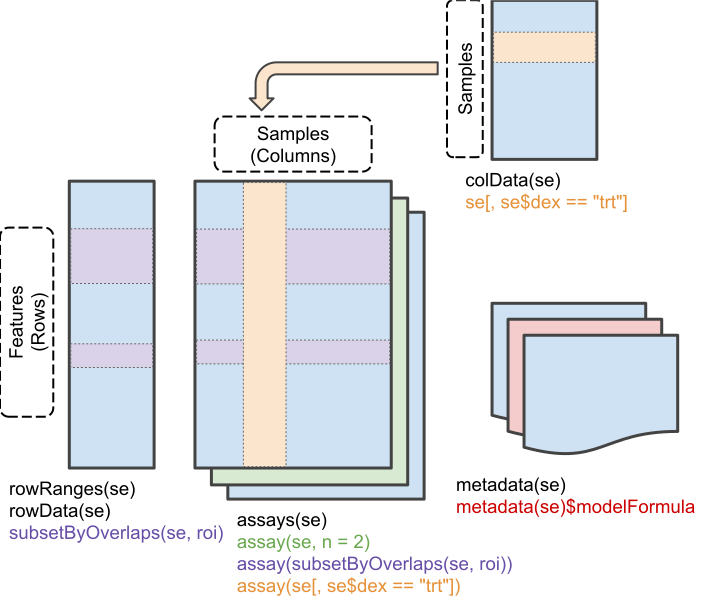
\includegraphics{SE.svg}
\caption{Summarized Experiment}
\end{figure}

\hypertarget{assays}{%
\subsection{Assays}\label{assays}}

The \texttt{airway} package contains an example dataset from an RNA-Seq
experiment of read counts per gene for airway smooth muscles. These data
are stored in a \texttt{RangedSummarizedExperiment} object which
contains 8 different experimental and assays 64,102 gene transcripts.

\begin{verbatim}
## Loading required package: airway
\end{verbatim}

\begin{Shaded}
\begin{Highlighting}[]
\KeywordTok{library}\NormalTok{(SummarizedExperiment)}
\KeywordTok{data}\NormalTok{(airway, }\DataTypeTok{package=}\StringTok{"airway"}\NormalTok{)}
\NormalTok{se <-}\StringTok{ }\NormalTok{airway}
\NormalTok{se}
\end{Highlighting}
\end{Shaded}

\begin{verbatim}
## class: RangedSummarizedExperiment 
## dim: 64102 8 
## metadata(1): ''
## assays(1): counts
## rownames(64102): ENSG00000000003 ENSG00000000005 ... LRG_98 LRG_99
## rowData names(0):
## colnames(8): SRR1039508 SRR1039509 ... SRR1039520 SRR1039521
## colData names(9): SampleName cell ... Sample BioSample
\end{verbatim}

To retrieve the experiment data from a \texttt{SummarizedExperiment}
object one can use the \texttt{assays()} accessor. An object can have
multiple assay datasets each of which can be accessed using the
\texttt{\$} operator. The \texttt{airway} dataset contains only one
assay (\texttt{counts}). Here each row represents a gene transcript and
each column one of the samples.

\begin{Shaded}
\begin{Highlighting}[]
\KeywordTok{assays}\NormalTok{(se)}\OperatorTok{$}\NormalTok{counts}
\end{Highlighting}
\end{Shaded}

\begin{longtable}[]{@{}lrrrrrrrr@{}}
\toprule
& SRR1039508 & SRR1039509 & SRR1039512 & SRR1039513 & SRR1039516 &
SRR1039517 & SRR1039520 & SRR1039521\tabularnewline
\midrule
\endhead
ENSG00000000003 & 679 & 448 & 873 & 408 & 1138 & 1047 & 770 &
572\tabularnewline
ENSG00000000005 & 0 & 0 & 0 & 0 & 0 & 0 & 0 & 0\tabularnewline
ENSG00000000419 & 467 & 515 & 621 & 365 & 587 & 799 & 417 &
508\tabularnewline
ENSG00000000457 & 260 & 211 & 263 & 164 & 245 & 331 & 233 &
229\tabularnewline
ENSG00000000460 & 60 & 55 & 40 & 35 & 78 & 63 & 76 & 60\tabularnewline
ENSG00000000938 & 0 & 0 & 2 & 0 & 1 & 0 & 0 & 0\tabularnewline
ENSG00000000971 & 3251 & 3679 & 6177 & 4252 & 6721 & 11027 & 5176 &
7995\tabularnewline
ENSG00000001036 & 1433 & 1062 & 1733 & 881 & 1424 & 1439 & 1359 &
1109\tabularnewline
ENSG00000001084 & 519 & 380 & 595 & 493 & 820 & 714 & 696 &
704\tabularnewline
ENSG00000001167 & 394 & 236 & 464 & 175 & 658 & 584 & 360 &
269\tabularnewline
\bottomrule
\end{longtable}

\hypertarget{row-regions-of-interest-data}{%
\subsection{`Row' (regions-of-interest)
data}\label{row-regions-of-interest-data}}

The \texttt{rowRanges()} accessor is used to view the range information
for a \texttt{RangedSummarizedExperiment}. (Note if this were the parent
\texttt{SummarizedExperiment} class we'd use \texttt{rowData()}). The
data are stored in a \texttt{GRangesList} object, where each list
element corresponds to one gene transcript and the ranges in each
\texttt{GRanges} correspond to the exons in the transcript.

\begin{Shaded}
\begin{Highlighting}[]
\KeywordTok{rowRanges}\NormalTok{(se)}
\end{Highlighting}
\end{Shaded}

\begin{verbatim}
## GRangesList object of length 64102:
## $ENSG00000000003 
## GRanges object with 17 ranges and 2 metadata columns:
##        seqnames            ranges strand |   exon_id       exon_name
##           <Rle>         <IRanges>  <Rle> | <integer>     <character>
##    [1]        X 99883667-99884983      - |    667145 ENSE00001459322
##    [2]        X 99885756-99885863      - |    667146 ENSE00000868868
##    [3]        X 99887482-99887565      - |    667147 ENSE00000401072
##    [4]        X 99887538-99887565      - |    667148 ENSE00001849132
##    [5]        X 99888402-99888536      - |    667149 ENSE00003554016
##    ...      ...               ...    ... .       ...             ...
##   [13]        X 99890555-99890743      - |    667156 ENSE00003512331
##   [14]        X 99891188-99891686      - |    667158 ENSE00001886883
##   [15]        X 99891605-99891803      - |    667159 ENSE00001855382
##   [16]        X 99891790-99892101      - |    667160 ENSE00001863395
##   [17]        X 99894942-99894988      - |    667161 ENSE00001828996
## 
## ...
## <64101 more elements>
## -------
## seqinfo: 722 sequences (1 circular) from an unspecified genome
\end{verbatim}

\hypertarget{column-sample-data}{%
\subsection{`Column' (sample) data}\label{column-sample-data}}

Sample meta-data describing the samples can be accessed using
\texttt{colData()}, and is a \texttt{DataFrame} that can store any
number of descriptive columns for each sample row.

\begin{Shaded}
\begin{Highlighting}[]
\KeywordTok{colData}\NormalTok{(se)}
\end{Highlighting}
\end{Shaded}

\begin{verbatim}
## DataFrame with 8 rows and 9 columns
##            SampleName     cell      dex    albut        Run avgLength
##              <factor> <factor> <factor> <factor>   <factor> <integer>
## SRR1039508 GSM1275862   N61311    untrt    untrt SRR1039508       126
## SRR1039509 GSM1275863   N61311      trt    untrt SRR1039509       126
## SRR1039512 GSM1275866  N052611    untrt    untrt SRR1039512       126
## SRR1039513 GSM1275867  N052611      trt    untrt SRR1039513        87
## SRR1039516 GSM1275870  N080611    untrt    untrt SRR1039516       120
## SRR1039517 GSM1275871  N080611      trt    untrt SRR1039517       126
## SRR1039520 GSM1275874  N061011    untrt    untrt SRR1039520       101
## SRR1039521 GSM1275875  N061011      trt    untrt SRR1039521        98
##            Experiment    Sample    BioSample
##              <factor>  <factor>     <factor>
## SRR1039508  SRX384345 SRS508568 SAMN02422669
## SRR1039509  SRX384346 SRS508567 SAMN02422675
## SRR1039512  SRX384349 SRS508571 SAMN02422678
## SRR1039513  SRX384350 SRS508572 SAMN02422670
## SRR1039516  SRX384353 SRS508575 SAMN02422682
## SRR1039517  SRX384354 SRS508576 SAMN02422673
## SRR1039520  SRX384357 SRS508579 SAMN02422683
## SRR1039521  SRX384358 SRS508580 SAMN02422677
\end{verbatim}

This sample metadata can be accessed using the \texttt{\$} accessor
which makes it easy to subset the entire object by a given phenotype.

\begin{Shaded}
\begin{Highlighting}[]
\CommentTok{# subset for only those samples treated with dexamethasone}
\NormalTok{se[, se}\OperatorTok{$}\NormalTok{dex }\OperatorTok{==}\StringTok{ "trt"}\NormalTok{]}
\end{Highlighting}
\end{Shaded}

\begin{verbatim}
## class: RangedSummarizedExperiment 
## dim: 64102 4 
## metadata(1): ''
## assays(1): counts
## rownames(64102): ENSG00000000003 ENSG00000000005 ... LRG_98 LRG_99
## rowData names(0):
## colnames(4): SRR1039509 SRR1039513 SRR1039517 SRR1039521
## colData names(9): SampleName cell ... Sample BioSample
\end{verbatim}

\hypertarget{experiment-wide-metadata}{%
\subsection{Experiment-wide metadata}\label{experiment-wide-metadata}}

Meta-data describing the experimental methods and publication references
can be accessed using \texttt{metadata()}.

\begin{Shaded}
\begin{Highlighting}[]
\KeywordTok{metadata}\NormalTok{(se)}
\end{Highlighting}
\end{Shaded}

\begin{verbatim}
## [[1]]
## Experiment data
##   Experimenter name: Himes BE 
##   Laboratory: NA 
##   Contact information:  
##   Title: RNA-Seq transcriptome profiling identifies CRISPLD2 as a glucocorticoid responsive gene that modulates cytokine function in airway smooth muscle cells. 
##   URL: http://www.ncbi.nlm.nih.gov/pubmed/24926665 
##   PMIDs: 24926665 
## 
##   Abstract: A 226 word abstract is available. Use 'abstract' method.
\end{verbatim}

Note that \texttt{metadata()} is just a simple list, so it is
appropriate for \emph{any} experiment wide metadata the user wishes to
save, such as storing model formulas.

\begin{Shaded}
\begin{Highlighting}[]
\KeywordTok{metadata}\NormalTok{(se)}\OperatorTok{$}\NormalTok{formula <-}\StringTok{ }\NormalTok{counts }\OperatorTok{~}\StringTok{ }\NormalTok{dex }\OperatorTok{+}\StringTok{ }\NormalTok{albut}

\KeywordTok{metadata}\NormalTok{(se)}
\end{Highlighting}
\end{Shaded}

\begin{verbatim}
## [[1]]
## Experiment data
##   Experimenter name: Himes BE 
##   Laboratory: NA 
##   Contact information:  
##   Title: RNA-Seq transcriptome profiling identifies CRISPLD2 as a glucocorticoid responsive gene that modulates cytokine function in airway smooth muscle cells. 
##   URL: http://www.ncbi.nlm.nih.gov/pubmed/24926665 
##   PMIDs: 24926665 
## 
##   Abstract: A 226 word abstract is available. Use 'abstract' method.
## 
## $formula
## counts ~ dex + albut
\end{verbatim}

\hypertarget{common-operations-on-summarizedexperiment}{%
\section{\texorpdfstring{Common operations on
\texttt{SummarizedExperiment}}{Common operations on SummarizedExperiment}}\label{common-operations-on-summarizedexperiment}}

\hypertarget{subsetting}{%
\subsection{Subsetting}\label{subsetting}}

\begin{itemize}
\tightlist
\item
  \texttt{{[}} Performs two dimensional subsetting, just like subsetting
  a matrix or data frame.
\end{itemize}

\begin{Shaded}
\begin{Highlighting}[]
\CommentTok{# subset the first five transcripts and first three samples}
\NormalTok{se[}\DecValTok{1}\OperatorTok{:}\DecValTok{5}\NormalTok{, }\DecValTok{1}\OperatorTok{:}\DecValTok{3}\NormalTok{]}
\end{Highlighting}
\end{Shaded}

\begin{verbatim}
## class: RangedSummarizedExperiment 
## dim: 5 3 
## metadata(2): '' formula
## assays(1): counts
## rownames(5): ENSG00000000003 ENSG00000000005 ENSG00000000419
##   ENSG00000000457 ENSG00000000460
## rowData names(0):
## colnames(3): SRR1039508 SRR1039509 SRR1039512
## colData names(9): SampleName cell ... Sample BioSample
\end{verbatim}

\begin{itemize}
\tightlist
\item
  \texttt{\$} operates on \texttt{colData()} columns, for easy sample
  extraction.
\end{itemize}

\begin{Shaded}
\begin{Highlighting}[]
\NormalTok{se[, se}\OperatorTok{$}\NormalTok{cell }\OperatorTok{==}\StringTok{ "N61311"}\NormalTok{]}
\end{Highlighting}
\end{Shaded}

\begin{verbatim}
## class: RangedSummarizedExperiment 
## dim: 64102 2 
## metadata(2): '' formula
## assays(1): counts
## rownames(64102): ENSG00000000003 ENSG00000000005 ... LRG_98 LRG_99
## rowData names(0):
## colnames(2): SRR1039508 SRR1039509
## colData names(9): SampleName cell ... Sample BioSample
\end{verbatim}

\hypertarget{getters-and-setters}{%
\subsection{Getters and setters}\label{getters-and-setters}}

\begin{itemize}
\tightlist
\item
  \texttt{rowRanges()} / (\texttt{rowData()}), \texttt{colData()},
  \texttt{metadata()}
\end{itemize}

\begin{Shaded}
\begin{Highlighting}[]
\NormalTok{counts <-}\StringTok{ }\KeywordTok{matrix}\NormalTok{(}\DecValTok{1}\OperatorTok{:}\DecValTok{15}\NormalTok{, }\DecValTok{5}\NormalTok{, }\DecValTok{3}\NormalTok{, }\DataTypeTok{dimnames=}\KeywordTok{list}\NormalTok{(LETTERS[}\DecValTok{1}\OperatorTok{:}\DecValTok{5}\NormalTok{], LETTERS[}\DecValTok{1}\OperatorTok{:}\DecValTok{3}\NormalTok{]))}

\NormalTok{dates <-}\StringTok{ }\KeywordTok{SummarizedExperiment}\NormalTok{(}\DataTypeTok{assays=}\KeywordTok{list}\NormalTok{(}\DataTypeTok{counts=}\NormalTok{counts),}
                              \DataTypeTok{rowData=}\KeywordTok{DataFrame}\NormalTok{(}\DataTypeTok{month=}\NormalTok{month.name[}\DecValTok{1}\OperatorTok{:}\DecValTok{5}\NormalTok{], }\DataTypeTok{day=}\DecValTok{1}\OperatorTok{:}\DecValTok{5}\NormalTok{))}

\CommentTok{# Subset all January assays}
\NormalTok{dates[}\KeywordTok{rowData}\NormalTok{(dates)}\OperatorTok{$}\NormalTok{month }\OperatorTok{==}\StringTok{ "January"}\NormalTok{, ]}
\end{Highlighting}
\end{Shaded}

\begin{verbatim}
## class: SummarizedExperiment 
## dim: 1 3 
## metadata(0):
## assays(1): counts
## rownames(1): A
## rowData names(2): month day
## colnames(3): A B C
## colData names(0):
\end{verbatim}

\begin{itemize}
\tightlist
\item
  \texttt{assay()} versus \texttt{assays()} There are two accessor
  functions for extracting the assay data from a
  \texttt{SummarizedExperiment} object. \texttt{assays()} operates on
  the entire list of assay data as a whole, while \texttt{assay()}
  operates on only one assay at a time. \texttt{assay(x,\ i)} is simply
  a convenience function which is equivalent to
  \texttt{assays(x){[}{[}i{]}{]}}.
\end{itemize}

\begin{Shaded}
\begin{Highlighting}[]
\KeywordTok{assays}\NormalTok{(se)}
\end{Highlighting}
\end{Shaded}

\begin{verbatim}
## List of length 1
## names(1): counts
\end{verbatim}

\begin{Shaded}
\begin{Highlighting}[]
\KeywordTok{assays}\NormalTok{(se)[[}\DecValTok{1}\NormalTok{]][}\DecValTok{1}\OperatorTok{:}\DecValTok{5}\NormalTok{, }\DecValTok{1}\OperatorTok{:}\DecValTok{5}\NormalTok{]}
\end{Highlighting}
\end{Shaded}

\begin{verbatim}
##                 SRR1039508 SRR1039509 SRR1039512 SRR1039513 SRR1039516
## ENSG00000000003        679        448        873        408       1138
## ENSG00000000005          0          0          0          0          0
## ENSG00000000419        467        515        621        365        587
## ENSG00000000457        260        211        263        164        245
## ENSG00000000460         60         55         40         35         78
\end{verbatim}

\begin{Shaded}
\begin{Highlighting}[]
\CommentTok{# assay defaults to the first assay if no i is given}
\KeywordTok{assay}\NormalTok{(se)[}\DecValTok{1}\OperatorTok{:}\DecValTok{5}\NormalTok{, }\DecValTok{1}\OperatorTok{:}\DecValTok{5}\NormalTok{]}
\end{Highlighting}
\end{Shaded}

\begin{verbatim}
##                 SRR1039508 SRR1039509 SRR1039512 SRR1039513 SRR1039516
## ENSG00000000003        679        448        873        408       1138
## ENSG00000000005          0          0          0          0          0
## ENSG00000000419        467        515        621        365        587
## ENSG00000000457        260        211        263        164        245
## ENSG00000000460         60         55         40         35         78
\end{verbatim}

\begin{Shaded}
\begin{Highlighting}[]
\KeywordTok{assay}\NormalTok{(se, }\DecValTok{1}\NormalTok{)[}\DecValTok{1}\OperatorTok{:}\DecValTok{5}\NormalTok{, }\DecValTok{1}\OperatorTok{:}\DecValTok{5}\NormalTok{]}
\end{Highlighting}
\end{Shaded}

\begin{verbatim}
##                 SRR1039508 SRR1039509 SRR1039512 SRR1039513 SRR1039516
## ENSG00000000003        679        448        873        408       1138
## ENSG00000000005          0          0          0          0          0
## ENSG00000000419        467        515        621        365        587
## ENSG00000000457        260        211        263        164        245
## ENSG00000000460         60         55         40         35         78
\end{verbatim}

\hypertarget{range-based-operations}{%
\subsection{Range-based operations}\label{range-based-operations}}

\begin{itemize}
\tightlist
\item
  \texttt{subsetByOverlaps()} \texttt{SummarizedExperiment} objects
  support all of the \texttt{findOverlaps()} methods and associated
  functions. This includes \texttt{subsetByOverlaps()}, which makes it
  easy to subset a \texttt{SummarizedExperiment} object by an interval.
\end{itemize}

In tne next code block, we define a region of interest (or many regions
of interest) and then subset our \texttt{SummarizedExperiment} by
overlaps with this region.

\begin{Shaded}
\begin{Highlighting}[]
\CommentTok{# Subset for only rows which are in the interval 100,000 to 110,000 of}
\CommentTok{# chromosome 1}
\NormalTok{roi <-}\StringTok{ }\KeywordTok{GRanges}\NormalTok{(}\DataTypeTok{seqnames=}\StringTok{"1"}\NormalTok{, }\DataTypeTok{ranges=}\DecValTok{100000}\OperatorTok{:}\DecValTok{1100000}\NormalTok{)}
\NormalTok{sub_se =}\StringTok{ }\KeywordTok{subsetByOverlaps}\NormalTok{(se, roi)}
\NormalTok{sub_se}
\end{Highlighting}
\end{Shaded}

\begin{verbatim}
## class: RangedSummarizedExperiment 
## dim: 74 8 
## metadata(2): '' formula
## assays(1): counts
## rownames(74): ENSG00000131591 ENSG00000177757 ... ENSG00000272512
##   ENSG00000273443
## rowData names(0):
## colnames(8): SRR1039508 SRR1039509 ... SRR1039520 SRR1039521
## colData names(9): SampleName cell ... Sample BioSample
\end{verbatim}

\begin{Shaded}
\begin{Highlighting}[]
\KeywordTok{dim}\NormalTok{(sub_se)}
\end{Highlighting}
\end{Shaded}

\begin{verbatim}
## [1] 74  8
\end{verbatim}

\hypertarget{constructing-a-summarizedexperiment}{%
\section{\texorpdfstring{Constructing a
\texttt{SummarizedExperiment}}{Constructing a SummarizedExperiment}}\label{constructing-a-summarizedexperiment}}

Often, \texttt{SummarizedExperiment} or
\texttt{RangedSummarizedExperiment} objects are returned by functions
written by other packages. However it is possible to create them by hand
with a call to the \texttt{SummarizedExperiment()} constructor. The code
below is simply to illustrate the mechanics of creating an object from
scratch. In practice, you will probably have the pieces of the object
from other sources such as Excel files or csv files.

Constructing a \texttt{RangedSummarizedExperiment} with a
\texttt{GRanges} as the \emph{rowRanges} argument:

\begin{Shaded}
\begin{Highlighting}[]
\NormalTok{nrows <-}\StringTok{ }\DecValTok{200}
\NormalTok{ncols <-}\StringTok{ }\DecValTok{6}
\NormalTok{counts <-}\StringTok{ }\KeywordTok{matrix}\NormalTok{(}\KeywordTok{runif}\NormalTok{(nrows }\OperatorTok{*}\StringTok{ }\NormalTok{ncols, }\DecValTok{1}\NormalTok{, }\FloatTok{1e4}\NormalTok{), nrows)}
\NormalTok{rowRanges <-}\StringTok{ }\KeywordTok{GRanges}\NormalTok{(}\KeywordTok{rep}\NormalTok{(}\KeywordTok{c}\NormalTok{(}\StringTok{"chr1"}\NormalTok{, }\StringTok{"chr2"}\NormalTok{), }\KeywordTok{c}\NormalTok{(}\DecValTok{50}\NormalTok{, }\DecValTok{150}\NormalTok{)),}
                     \KeywordTok{IRanges}\NormalTok{(}\KeywordTok{floor}\NormalTok{(}\KeywordTok{runif}\NormalTok{(}\DecValTok{200}\NormalTok{, }\FloatTok{1e5}\NormalTok{, }\FloatTok{1e6}\NormalTok{)), }\DataTypeTok{width=}\DecValTok{100}\NormalTok{),}
                     \DataTypeTok{strand=}\KeywordTok{sample}\NormalTok{(}\KeywordTok{c}\NormalTok{(}\StringTok{"+"}\NormalTok{, }\StringTok{"-"}\NormalTok{), }\DecValTok{200}\NormalTok{, }\OtherTok{TRUE}\NormalTok{),}
                     \DataTypeTok{feature_id=}\KeywordTok{sprintf}\NormalTok{(}\StringTok{"ID%03d"}\NormalTok{, }\DecValTok{1}\OperatorTok{:}\DecValTok{200}\NormalTok{))}
\NormalTok{colData <-}\StringTok{ }\KeywordTok{DataFrame}\NormalTok{(}\DataTypeTok{Treatment=}\KeywordTok{rep}\NormalTok{(}\KeywordTok{c}\NormalTok{(}\StringTok{"ChIP"}\NormalTok{, }\StringTok{"Input"}\NormalTok{), }\DecValTok{3}\NormalTok{),}
                     \DataTypeTok{row.names=}\NormalTok{LETTERS[}\DecValTok{1}\OperatorTok{:}\DecValTok{6}\NormalTok{])}

\KeywordTok{SummarizedExperiment}\NormalTok{(}\DataTypeTok{assays=}\KeywordTok{list}\NormalTok{(}\DataTypeTok{counts=}\NormalTok{counts),}
                     \DataTypeTok{rowRanges=}\NormalTok{rowRanges, }\DataTypeTok{colData=}\NormalTok{colData)}
\end{Highlighting}
\end{Shaded}

\begin{verbatim}
## class: RangedSummarizedExperiment 
## dim: 200 6 
## metadata(0):
## assays(1): counts
## rownames: NULL
## rowData names(1): feature_id
## colnames(6): A B ... E F
## colData names(1): Treatment
\end{verbatim}

A \texttt{SummarizedExperiment} can be constructed with or without
supplying a \texttt{DataFrame} for the \emph{rowData} argument:

\begin{Shaded}
\begin{Highlighting}[]
\KeywordTok{SummarizedExperiment}\NormalTok{(}\DataTypeTok{assays=}\KeywordTok{list}\NormalTok{(}\DataTypeTok{counts=}\NormalTok{counts), }\DataTypeTok{colData=}\NormalTok{colData)}
\end{Highlighting}
\end{Shaded}

\begin{verbatim}
## class: SummarizedExperiment 
## dim: 200 6 
## metadata(0):
## assays(1): counts
## rownames: NULL
## rowData names(0):
## colnames(6): A B ... E F
## colData names(1): Treatment
\end{verbatim}

\hypertarget{sessioninfo}{%
\section{sessionInfo()}\label{sessioninfo}}

\begin{Shaded}
\begin{Highlighting}[]
\KeywordTok{sessionInfo}\NormalTok{()}
\end{Highlighting}
\end{Shaded}

\begin{verbatim}
## R version 3.5.0 RC (2018-04-16 r74624)
## Platform: x86_64-apple-darwin15.6.0 (64-bit)
## Running under: macOS Sierra 10.12.6
## 
## Matrix products: default
## BLAS: /Library/Frameworks/R.framework/Versions/3.5/Resources/lib/libRblas.0.dylib
## LAPACK: /Library/Frameworks/R.framework/Versions/3.5/Resources/lib/libRlapack.dylib
## 
## locale:
## [1] en_US.UTF-8/en_US.UTF-8/en_US.UTF-8/C/en_US.UTF-8/en_US.UTF-8
## 
## attached base packages:
## [1] parallel  stats4    stats     graphics  grDevices utils     datasets 
## [8] methods   base     
## 
## other attached packages:
##  [1] airway_0.114.0              SummarizedExperiment_1.9.18
##  [3] DelayedArray_0.5.35         BiocParallel_1.13.3        
##  [5] matrixStats_0.53.1          Biobase_2.39.2             
##  [7] GenomicRanges_1.31.23       GenomeInfoDb_1.15.5        
##  [9] IRanges_2.13.29             S4Vectors_0.17.43          
## [11] BiocGenerics_0.25.3        
## 
## loaded via a namespace (and not attached):
##  [1] Rcpp_0.12.16           knitr_1.20             XVector_0.19.9        
##  [4] magrittr_1.5           zlibbioc_1.25.0        lattice_0.20-35       
##  [7] highr_0.6              stringr_1.3.1          tools_3.5.0           
## [10] grid_3.5.0             htmltools_0.3.6        yaml_2.1.19           
## [13] rprojroot_1.3-2        digest_0.6.15          Matrix_1.2-14         
## [16] GenomeInfoDbData_1.1.0 bitops_1.0-6           RCurl_1.95-4.10       
## [19] evaluate_0.10.1        rmarkdown_1.9          stringi_1.2.2         
## [22] compiler_3.5.0         backports_1.1.2
\end{verbatim}


\end{document}
